\documentclass[a4j,10pt,dvipdfmx]{jarticle}
\usepackage{siunitx}
\usepackage[dvipdfmx]{graphicx}
\usepackage{pdfpages}
\usepackage{here}
\usepackage{listings,jlisting}
\usepackage{tabularx}
\lstset{
  basicstyle={\ttfamily},
  identifierstyle={\small},
  commentstyle={\smallitshape},
  keywordstyle={\small\bfseries},
  ndkeywordstyle={\small},
  stringstyle={\small\ttfamily},
  frame={tb},
  breaklines=true,
  columns=[l]{fullflexible},
  numbers=left,
  xrightmargin=0zw,
  xleftmargin=3zw,
  numberstyle={\scriptsize},
  stepnumber=1,
  numbersep=1zw,
  lineskip=-0.5ex
}
\begin{document}
\title{非線形方程式の課題}
\author{学籍番号2120029, 氏名 政野玄空}
\date{2023年7月14日}
\maketitle
\section{二分法}
\subsection{1}
穴埋め箇所1
\begin{itemize}
  \item 穴埋め箇所1: (b-a)/n
  \item 穴埋め箇所2: x-h
  \item 穴埋め箇所3: f(a)*f(c)
  \item 穴埋め箇所4: (a+b)/2.0
  \item 穴埋め箇所5:  pow(x,5)-(5*pow(x,3))+(4*x)
\end{itemize}
\subsection{2}
1で穴埋めした出力結果をスクリーンショットを示す.
\begin{figure}[H]
  \begin{center}
  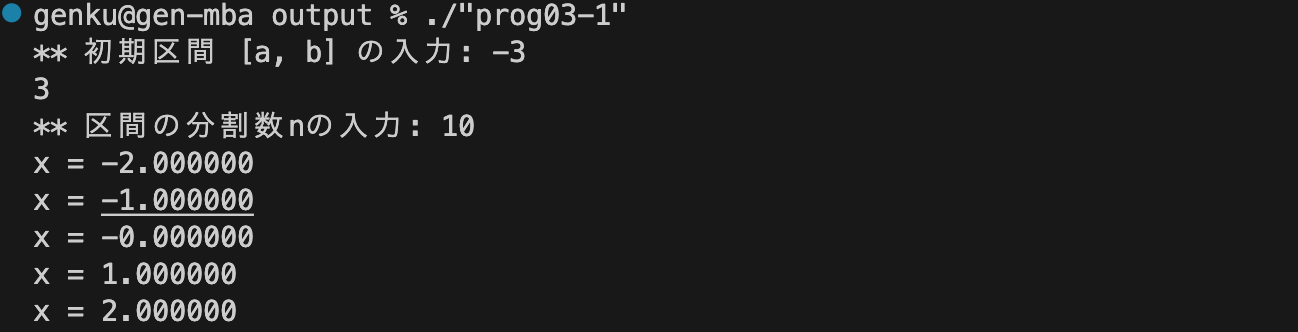
\includegraphics[height=7cm,width=10cm]{screen714.png}
  \caption{prog03-1.cを1の通りに埋めて初期区間a,bを-3,3,区間の分割数nの入力10を入力した結果}
\end{center}
\end{figure}
-2.0,-1.0,0.0,1.0,2.0の結果が得られた.
\section{ニュートン法}
\subsection{1}
$x^{3} - 3x^{2} - x + 3 = 0$ をニュートン法を用いて解くプログラムを作成した.
\begin{lstlisting}[label=prm1, caption=newton.c]
  #include <stdio.h>
  #include <math.h>
  #include <stdlib.h>
  
  double newton(double x, double m, double p);
  double f(double x);
  double df(double x);
  
  int main(void)
  {
    double x, max = 100000 ,eps = pow(2.0, -30.0);
  
    printf("** 初期値の入力: ");
    scanf("%lf", &x);
  
    printf("x = %lf\n", newton(x, max, eps));
  
    return (0);
  }
  /* newton */
  double newton(double x, double m, double p)
  {
    double n = 0;
    double d;
    do{
      d= -f(x)/df(x);
      x = x + d;
      n++;
    } while (fabs(d) > p && n < m);
    if (n == m) {
      printf("failed");
      exit(0);
    } else {
      return x;
    }
  }
  
  /* 関数の定義 */
  double f(double x)
  {
    return pow(x,3)+(-3*pow(x,2))+(-1*x)+3;
  }
  /* 関数の微分 */
  double df(double x)
  {
    return (3*pow(x,2))+(-6*x)+(-1);
  }  
\end{lstlisting}
\subsection{2}
1のコードの初期値を-2,1.5,5.0にした結果のスクリーンショットを示す.
\begin{figure}[H]
  \begin{center}
  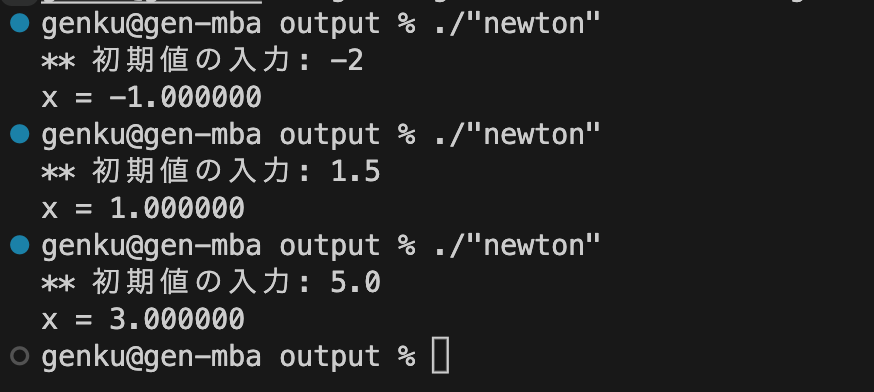
\includegraphics[height=7cm,width=10cm]{screen716.png}
  \caption{newton.cの初期値を-2,1.5,5.0にした結果}
\end{center}
\end{figure}
$x^{3} - 3x^{2} - x + 3 = 0$ をニュートン法を用いて初期値を-2,1.5,5.0にして解いた結果は-1.0,1.0,3.0となることを確認した.
\section{考察課題}
\subsection{ニュートン法で初期値を2.1547,-0.1547としたとき,解が求まらない理由}
自身で設定したMaxの値では求まってしまうので数値を100,50と下げて確認してみると50で失敗した.
ヒント通り$x^{3} - 3x^{2} - x + 3 = 0$の増減表を書き出してみる.解の公式よりxは$\frac{-2\sqrt{3}+3}{3}$,$\frac{2\sqrt{3}+3}{3}$となる.$\sqrt{3}$は1.73205で計算してみると-0.1547,2.1547になる.

\begin{center}
  \begin{tabular}{|c||ccccc|}
  \hline
  $x$ & $\cdots$ & $-0.1547$ & $\cdots$ & $2.1547$ & $\cdots$ \\
  \hline
  $f'(x)$ & $+$ & $0$ & $-$ & $0$ & $+$ \\
  \hline
  $f(x)$ & $\nearrow$ & & $\searrow$ & & $\nearrow$ \\
  \hline
  \end{tabular}
  \end{center}
このことより-0.1547,2.1547を初期値として入力すると算出したいxから最も離れた位置になってしまい,試行回数によっては収束しなくなると考えられる.
\subsection{proc03-1.cのmain関数内のfor文をfor (x=a+h; x != b; x+=h) とするとプログラムが停止しなくなる理由}
まずこのようにプログラムを変更してhの値と変化するxの値,xがbを上回った地点をデバックしてみる.またfor文の中にx==bのときのデバックも仕込んでみる.
\begin{verbatim}
genku@gen-mba output % ./"prog03-1"
** 初期区間 [a, b] の入力: -3
3
** 区間の分割数nの入力: 10
h = 0.600000
x = -2.400000
x = -1.800000
x = -2.000000
x = -1.200000
x = -0.600000
x = -1.000000
x = 0.000000
x = -0.000000
x = 0.600000
x = 1.200000
x = 1.000000
x = 1.800000
x = 2.400000
x = 2.000000
x > b 3.000000
x = 3.000000
x > b 3.600000
x = 3.600000
^C
\end{verbatim}
見た限りではxは3.000000のときがありループから抜けれそうではあるが実際は題意の通りそうはならない.x==bのときはfor文を抜けるので当然デバックもされない.
適当にdoubleの数値を入力して比較するプログラムを作ってみる.
\begin{lstlisting}[label=sam, caption=sample1.c]
#include <stdio.h>
#include <math.h>

int main(void)
{
  double a, b;
  scanf("%lf %lf", &a, &b);
  if (a == b) {
    printf("a==b");
  }
  return (0);
}
\end{lstlisting}
\begin{verbatim}
genku@gen-mba output % ./"test"
3
3
a==b%
\end{verbatim}
この結果からdoubleの計算のなかでなんらかの誤差が発生しているのではないかと考えられる.プログラムのなかの計算だけを抜き出してみるとこのようになる.
\begin{lstlisting}[label=sam2, caption=sample2.c]
#include <stdio.h>
#include <math.h>

int main(void)
{
  double a= -3,b= 3,n= 10,x,h;
  h= (b-a)/n;
  x = a;
  for(int i = 0; i < 10; i++){
    x+=h;
  }
  printf("x = %lf b = %lf",x,b);
  if(b==x) {
    printf("success");
  }
  return (0);
}
\end{lstlisting}
実行結果はこのようになり同値だが"success"の表記はされない.
\begin{verbatim}
genku@gen-mba output % ./"test"
x = 3.000000 b = 3.000000%  
\end{verbatim}
ここでhを計算せず0.6を代入してみる.しかし結果は変わらなかった. 0.6という数字になんらかの原因があると思われる.
ここで0.6を2進数表記で表してみると0.100110011..と無限に続いていくことがわかる.double型は32bitなのでその中に収めなければいけなくどこかで丸める必要が出てくる.コンピュータで計算するには2進数にする必要があるので0.6という数字はそのままではおいておくことのできない数字ということがわかる.
その丸められた無視で切るような誤差が10回繰り返して足し算をするうちに無視できない誤差になり同値のように見えるがプログラム上ではイコールにならないと考察できる.

試しに変数に代入した0.6と0.6を比較してみる.doubleより精度の低いfloatで試してみる.
\begin{lstlisting}[label=sam3, caption=sample3.c]
#include <stdio.h>
#include <math.h>

int main(void)
{
  float h = 0.6;
  if (h == 0.6) {
    printf("success");
  }
  printf("%lf",h);
  return (0);
}
\end{lstlisting}
実行結果はこのようになる.代入した途端から数値に誤差が発生してしまっている.
\begin{verbatim}
  genku@gen-mba output % ./"test"
  0.600000%     
\end{verbatim}
よってx == bにならない理由は0.6をdouble型におさめるときに丸めた誤差が繰り返しの処理によって無視できなくなるものになっているからと言える.
\end{document}
